%liste des modules réalisés
%Preuve du fonctionnement de chaque module

\subsection{Extraction du texte des documents}
Le module d'extraction de texte se présente sous la forme d'un script Bash pouvant être lancé sur l'intégralité du contenu d'un dossier.
Notre script va lire les documents contenus dans le dossier un par uns et écrire dans un dossier de sortie un nouveau fichier contenant le texte d'un des documents analysé.
Les résultats ont également été stockés sur \href{https://github.com/smallito/PFE/tree/master/codes/transcripts}{GitHub}.

Pour ce module, nous avons commencé par étudier les différents types de documents que nous pouvions trouver:
\begin{itemize}
\item PDF full text
\item PDF scanné
\item PDF mixte
\item PDF compressé
\item autres formats (DOCX, OBS, \ldots)
\end{itemize}

\subsubsection{PDF full text}
Le type de document que nous observons le plus souvent est le document PDF full text.
Le texte de celui ci est assez facile à extraire: on peut utiliser un programme commun comme pdftotext qui renverra directement le contenu textuel d'un PDF dans un nouveau fichier.

Si le nombre de caractères présents dans le document est inférieur à un certain seuil (une dizaines de caractères), on considère que le texte n'a pas été extrait et que le document doit être considéré comme un PDF scanné.

\subsubsection{PDF scanné}
Le PDF scanné ne contient pas directement de texte inscrit.
Il se présente comme une suite d'images scannées, dans notre cas de scans d'un document.
La raison pour laquelle un document PDF est scanné plutôt que full text est très généralement due à une signature ou un tampon que la prefecture a jugé nécessaire d'inclure.

Pour lire ce type de document, nous avons mis en place un système d'OCR (Optical Character Recognition) appelé Tesseract pour extraire visuellement les caractères.
Tesseract est l'état de l'art de l'OCR open source mais ne peux pas être utilisé tel quel et donner d'excellents résultats: il possède de nombreux paramètres et spécifications qui permettent de maximiser les résultats pour des cas d'utilisation spécifiques.

Afin d'évaluer la performance de notre OCR, nous avons mis en place une méthode d'évaluation de performances basée sur deux paramètres: la proximité du transcript par rapport à la sortie de l'OCR et la présence de certains termes d'importance (voir~\ref{testOCR} pour le détail des méthodes de test).

Les performances de l'OCR ainsi paramétré se sont révélées insuffisantes.
Le score de proximité et le score de mots clefs étaient tout deux en dessous de 70\%.


Pour améliorer ce score, nous avons effectué un traitement d'image sur le document avant de l'envoyer dans le système d'OCR\@.

Le processus de traitement se déroule comme suit:
\begin{itemize}
\item Le document est découpé en pages stockées en format TIF
\item Chaque page est traitée individuellement par des méthodes de seuillage, ouverture, fermeture, floutage, \ldots
\item L'ensemble des pages traitées est rassemblé en une seule image TIFF, format adapté à Tesseract
\end{itemize}

La méthode de traitement a également été optimisée avec les tests mentionnés précédemment (voir~\ref{testOCR}).

Le résultat final est bien plus satisfaisant que les premiers résultats de 70\%: nos nouveaux scores se situent autour de 85\% de précision pour les mots clefs et 88\% pour le score de proximité.

\begin{figure}[h!]
  \centering
  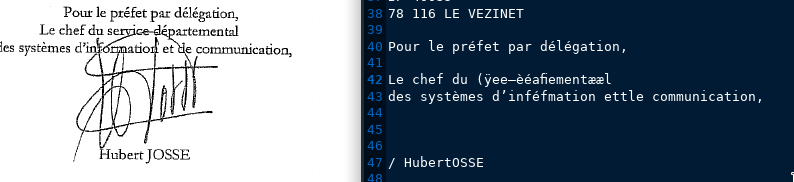
\includegraphics[width=0.7\textwidth]{pbsOCR.png}
	\caption[]{Exemple des défauts de l'OCR avec les signatures}
	\label{fig:defautsOCR}
\end{figure}

Cette méthode n'est cependant pas parfaite: de nombreux `e' se transforment en `c' par exemple, et les tampons et signatures ne sont pas reconnus comme du texte et provoquent l'apparition de caractères spéciaux au milieu du transcrit (exemple ci dessus).

Les résultats ont été jugés suffisants en accord avec le commanditaire, l'extraction de texte par OCR n'étant pas le sujet principal du PFE\@.

\subsubsection{PDF mixte}
Certains PDFs peuvent également être des PDF full text contenant une ou deux pages scannées.
Ce type de PDF est simplement considéré comme un PDF full text par notre programme, nous n'avons pas eu le temps de mettre en place une méthode d'extraction pour ce cas particulier, de toute façon assez rare.

Une méthode pour s'occuper d'un document de ce genre serait de découper le document d'entré par pages avant d'en extraire le texte individuellement, afin de détecter quel page ne contient pas de texte et l'envoyer à l'OCR\@.

Cette méthode nécessiterait cependant une refonte du script et serait plus longue à l'exécution.

\subsubsection{Récupération des données d'importance}
Nos test expérimentaux ont également mis en valeur un type de PDF ne contenant qu'un texte très court conseillant d' "obtenir `un lecteur de PDF' pour pouvoir ouvrir un document de ce type".

Après discussion avec notre commanditaire, nous avons découvert que ce type de stockage avait été utilisé entre les années 2014 et 2016, et représentait donc une part non négligeable de nos documents d'étude.

Ce type de format est en fait un format de PDF similaire sur le principe au format TIFF pour les images: il s'agit d'un PDF contenant une suite de PDF individuels.
Nous avons donc utilisé un programme de décompression de PDF pour en sortir les PDF inclus, puis un autre programme permettant de recréer un seul PDF avec tous les PDF extrais précédemment.
Ce nouveau PDF peut ainsi être fourni directement à l'extracteur de texte pour en récupérer le transcript.

\subsubsection{Autres formats}
Il arrive rarement que le document d'entrée soit d'un format différent que PDF, mais cette possibilité existe.
Pour ne pas exclure ces documents sans pour autant développer des solutions dédiées (ce qui aurait pris beaucoup de temps), nous avons réglé pdftotext pour qu'il tente d'effectuer une conversion en PDF du document avant de le traiter normalement.
Si cette étape échoue, le document est simplement ignoré.



\subsection{Extraction des données spécifiques}
Une fois le transcript obtenu, l'extraction des données du document peut commencer.
La listes des données d'importance a été déterminée avec le commanditaire (Liste des informations: voir~\ref{infosImp}).
Nous avons séparé ces données d'importance en deux catégories:
\begin{itemize}
\item Données respectant une norme de notation stricte ou presque stricte.\newline
Par exemple, les références de RAA ont toujours le même format: numéroDuDépartement-année-indice
\item Données non normées.\newline
Ces données n'ont pas de format spécifique défini.
Par exemple, un nom propre.
\end{itemize}

Les données normées sont bien plus faciles à repérer que les données non normées dans un texte car les formats qu'elles présentent sont similaires.

\subsubsection{Données normées}
%dates, raa, arretes, articles, lois, decrets, titres
Afin de trouver les données normées de chaque document, nous avons utilisé des RegEx (Regular Expression).

Un RegEx est une suite de caractères qui décrit un ensemble de chaines de caractères selon une syntaxe précise.
Cette méthode est extrêmement fiable et rapide à l'exécution, mais elle demande beaucoup de travail d'analyse pour bien inclure toutes les informations désirées, et présente le désavantage majeur d'être très rigide.
Un RegEx est en effet purement logique, ses frontières de détection sont très rigides et il suffit d'un petit écart de format pour que l'information ne soit pas récupérée.
Le RegEx est également absolument mécanique: Tout résultat qui correspond au pattern sera gardé, peut importe sa pertinence, ce qui nous oblige à faire passer nos résultats par une étape de tri et de filtrage par la suite.

L'utilisation des RegEx nous a demandé beaucoup de travail, la syntaxe étant quelque peu complexe.

Pour retrouver une donnée normée comme un numéro de RAA, on peut décomposer sa forme générale: 53-2019-010 par exemple, se décompose en deux chiffres, un tiret, 4 chiffres, tiret, 3 chiffres.
Un RegEx basique peut facilement retrouver ce numéro dans l'ensemble du texte, mais ne prendra pas en compte un numéro de la forme 053-2019-010 à cause du 0 au début.

Nous avons donc conduit une étude de toutes les variations de notation pouvant exister pour nos termes à rechercher.
Ces résultats nous ont permis de créer des RegEx adaptés à la plupart des cas particuliers rencontrés.
Nous avons donc crée au moins un pattern RegEx pour chaque information normée.

\begin{figure}[h!]
  \centering
  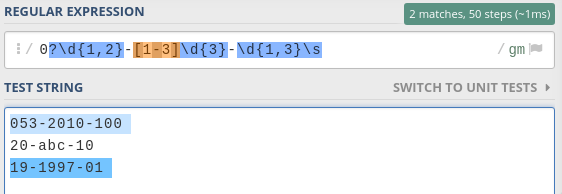
\includegraphics[width=0.7\textwidth]{regex_RAA.png}
	\caption[]{RegEx pour les numéros de RAA et exemples de détection}
	\label{fig:regexRAA}
\end{figure}

Certains des RegEx développés sont bien plus complexes que celui de l'image~\ref{fig:regexRAA}.

Les numéros d'arrêtés, de décrets et de lois ont été bien plus difficiles à différencier car ils ont une syntaxe similaire.
Ces RegEx se basent sur le mot précédent le numéro détecté pour déterminer sa catégorie (arrêté, décret ou lois).


L'extraction des titres des arrêtés a également été réalisée avec des RegEx.

Cette détection était la plus difficile car cette fois il ne suffit pas de trouver un pattern de nombres ou quelques caractères mais des phrases entières, sans format particulier.
Nos observations sur les documents ont montrés que les titres commençaient toujours par `arrêté' et pouvaient finir par `arrêté', `article', `préfet', \ldots

Le RegEx est dans ce cas bien plus complexe que les autres et l'ensemble des titres du document sont renvoyés, mais n'est pas parfait: certains titres sont des morceaux de texte sans grand intérêt, répétitifs, vides, \ldots
Les titres d'arrêtés sont donc traités bien plus en profondeur que les autres informations.
L'image~\ref{fig:regexTitles} montre quelques résultats de titres nettoyés d'un document par RegEx.

\begin{figure}[h!]
  \centering
  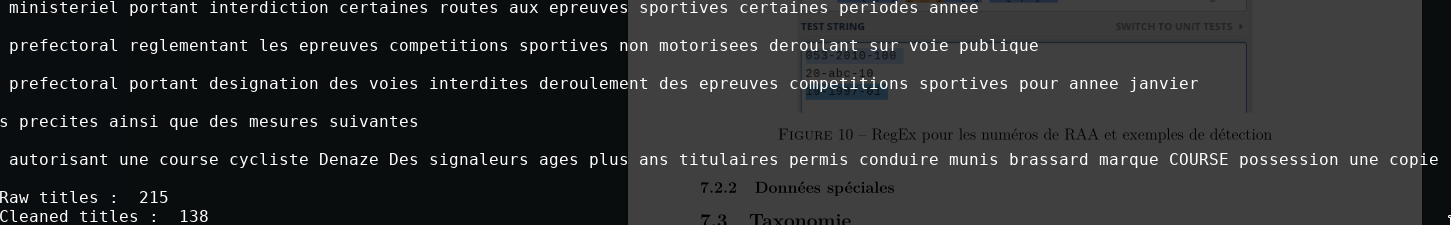
\includegraphics[width=0.7\textwidth]{title_results.png}
	\caption[]{Titres avant et après nettoyage}
	\label{fig:regexTitles}
\end{figure}

On peut remarquer que le nombre de titres passe de 215 à 138 après nettoyage.
Cette étape permet donc de gagner beaucoup de place de stockage de métadonnées et de temps de recherche d'informations dans les titres (comme la taxonomie).


La detection des dates est aussi gérée par RegEx.
Il existe deux formats principaux de dates: le format `jour/mois/année' et le format `jour mois année' (en lettres).
Ces deux patterns sont reconnus par des RegEx distincts, puis transformés en format unique `année-mois-jour' afin de pouvoir facilement trier les documents par date et de ne pas mélanger les formats de stockage.

C'est lors de la transformation en format unique qu'on peut détecter si le RegEx ne nous a pas renvoyé une date valable.
Pour le moment, cette date invalide est simplement ignorée, mais une future version du programme pourrait utiliser une méthode comme la distance de Levenshtein ou un Word2Vec pour reconnaitre si la date est mal écrite ou invalide.




\subsubsection{Données spéciales}
%noms propres, lieux, orgs
La recherche des données non normée est une tâche pour laquelle on ne peux pas utiliser de RegEx.
Les noms et prénoms ne suivent pas de règle de notation particulière pour les différencier du reste du texte, tout comme les noms de lieux et d'organisation.


Pour trouver ces informations dans le texte, nous avons utilisé une librairie python nommé Spacy offrant des fonctions avancées de NLP\@.
Spacy analyse le transcript en nous renvoyant des ensembles de mots classés selon le model.


\begin{figure}[h!]
  \centering
  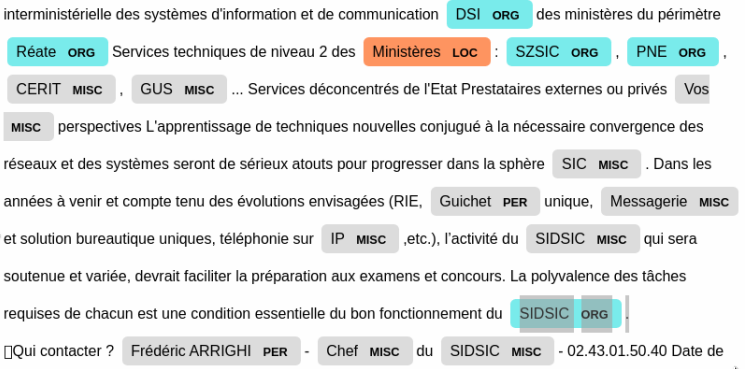
\includegraphics[width=0.7\textwidth]{spacyNLP.png}
	\caption[]{Catégories de Spacy}
	\label{fig:spacyNLP}
\end{figure}

Comme montré dans l'image~\ref{fig:spacyNLP}, Spacy analyse plusieurs catégories:
\begin{itemize}
\item LOC\@: Lieux
\item ORG\@: organisation
\item PER\@: personne
\item MISC\@: non défini
\end{itemize}

Ces catégories correspondent assez bien à ce que nous recherchons, même si les résultats ne sont pas exacts.
La précision des résultats peut être améliorée en utilisant un plus gros modèle préentrainé.

Cependant les modèles préentrainés Français sont assez peu répandus, et un plus gros modèle entraine un temps de chargement et d'exécution du modèle bien plus long.
Pour notre POC, le modèle Français de taille medium suffit amplement.

Des méthodes de filtrage/nettoyage ont toutefois été mise en place avec des RegEx afin de supprimer les erreurs majeures.

\subsection{Taxonomie}%Martin
\subsubsection{Approche par Word2Vec\label{word2vecReal}}
Pour extraire la taxonomie des documents, nous avons débuté par une approche basée sur des \textit{\gls{embed}} construits grâce à un réseau Word2Vec entrainé sur un corpus français.
Idéalement, ce réseau nous permettrait d'obtenir des taxonomies en comparant les mots du documents avec ceux présents dans la liste de taxonomies (sous forme de vecteurs), et d'ajouter les mots dont la distance, définie en (~\ref{eq:distCosine}), est sous un seuil.
Cette approche, ne nécessitant pas de corpus annoté semblait correspondre à nos besoins, même si il n'existe pas de cas dans la littérature scientifique ou elle a été appliquée avec succès. %Réecrire...


Les failles décelées par l'implémentation de cette méthode sont les suivantes.

Premièrement, le temps d'exécution de cette méthode pour un seul document était bien trop long pour imaginer un test sur nos 431 documents.
En effet, un document administratif est par nature très verbeux, et donc long.

La majorité du texte ne nous est cependant pas nécessaire pour une analyse taxonomique; 
il sert en effet à donner un contexte précis pour le lecteur et ne donne pas forcément plus d'information concernant le sujet du document en lui même que le titre du document en question, qui contient souvent toutes les informations taxonomiques nécéssaires. 


Deuxièmement, nous n'avons pas pu obtenir les résultats taxonomiques escomptés.
Le principal obstacle venant du fait que les mots de la taxonomie peuvent être en fait des phrases, ou tout du moins de multiples mots dont les sens ne sont pas forcément corrélés.

Par exemple, `Outre mer', `fromage au lait cru', `Pays de la Loire', \ldots et le très utilisé `Délégation de signature' sont des termes de la taxonomie composés de plusieurs mots dont le sens n'est pas proche.

Word2Vec, que nous utilisions pour obtenir les \textit{embeddings}, ne fonctionne bien que pour des mots uniques et pas sur des \textit{groupes de mots} ou \textit{n-grammes}.
Doc2vec, qui lui peut fonctionner sur des n-grammes, voir des paragraphes ou documents entiers, a besoin d'être entrainé sur des documents labellisés qui lui apporteront le contexte nécessaire pour former des \textit{embeddings} cohérents.


Cependant, la taxonomie donne un context très difficile à analyser pour un programme.
Il s'agit seulement d'une liste de mots et de phrasez ordonnée sous la forme d'un arbre (voir figure~\ref{fig:tree}).
Cette disposition rend l'utilisation d'un Doc2Vec très inconventionnelle, et les test que nous avons mené n'ont pas donné de résultats.


Nous tout d'abord amélioré la rapidité d'exécution en précalculant les vecteurs de la taxonomie.
Initialement, nous itérions simplement sur la liste de taxonomies, et calculions les \textit{embeddings} à la volée.
En calculant les vecteurs \textit{embedding} avant même l'exécution du module de détection de taxonomie, avons économisé une dizaine de secondes par documents.
Ensuite, plutôt que de traiter l'intégralité du texte avec Word2Vec, nous avons utilisé que les titres des arrêtés du RAA, qui peuvent constituer à eux seuls un résumé du RAA\@.
Ainsi, la quantité de texte à analyser est grandement réduite et une dizaine de secondes d'analyse supplémentaire sont gagnées par documents.

Pour essayer de contrer le problème des mauvais résultats, nous avons transformé chaque mot de la phrase en sa racine par le procédé dit la \textit{lemmatisation} à l'aide de la librairie Spacy\cite{spacy}.
Nous avons également filtré les \textit{stopwords} du texte à analyser.
Les \textit{stopwords} sont des mots très fréquemment dans les phrases, comme les déterminants, transformant la phrase `médecine physique et de réadaptation' en `médecine physique réadaptation'.
On utilise ensuite un Word2Vec sur chaque mot de la taxonomie est du titre pour obtenir plusieurs vecteurs.
Pour obtenir un seul vecteur que nous comparerons avec les mots du documents, nous effectuons un simple moyennage entre les valeurs de chaque mot de la phrase.


Ces modifications ont améliorés significativement les performances en temps du programme et la pertinence des taxonomies obtenues.
Cependant, les taxonomies obtenues à l'aide de ce système n'étais pas encore d'une qualité suffisante pour nos standards.
Les taxonomies monotermes étaient bien mieux détectées mais les multitermes restaient inutilisées.


Ce dysfonctionnement est du à la manière dont nous utilisons les vecteurs de mots produit par Word2Vec: une comparaison simple, ne donnant qu'une métrique de similarité ne suffit pas à établir un contexte suffisant pour ajouter des taxonomies sensées.
En effet, si un mot dans un titre et un mot dans la taxonomie sont identiques, alors leur métrique sera forcément faible (ils seront considérés comme ayant un sens proche), même si ces deux mots sont utilisés différemment dans le contexte actuel.
On peut prendre l'exemple du terme `montant': il peut avoir la signification d'un nombre, une action, un élément d'une porte, \ldots

On se retrouve alors à obtenir une grande quantités de termes taxonomiques qui ne sont pas pertinentes.
De plus, la question de la rapidité d'analyse n'as pas pu être totalement élucidée, même avec un prétraitement des vecteurs et l'utilisation des titres plutôt que du texte entier.
Pour un seul document, on pouvait avoir jusqu'à plusieurs dizaines de secondes de calcul pour la seule taxonomie.
Même si l'optimisation n'était pas une priorité dans ce projet, il devenait évident que cette approche ne fonctionnerait pas dans les délais impartis.


\subsubsection{Approche par détection de mots commun}
La solution donnant les meilleurs résultats fut d'extraire les titres d'arrêtées administratifs, qui sont les principaux constituants des RAA à classer, les traiter par lemmatisation et élimination des stopwords, puis d'effectuer une recherche des mots communs dans la taxonomie.
Si un terme lemmatisé de la taxonomie se trouve dans le titre de l'article administratif, alors celui ci est ajouté au document.
Cette solution est non seulement bien plus simple, mais permet également de vérifier la qualité des résultats plus aisément qu'à l'aide d'un \textit{embedding}, et elle est bien plus rapide, permettant l'analyse d'un document entier en quelques secondes à peine.

\begin{figure}[h!]
  \centering
  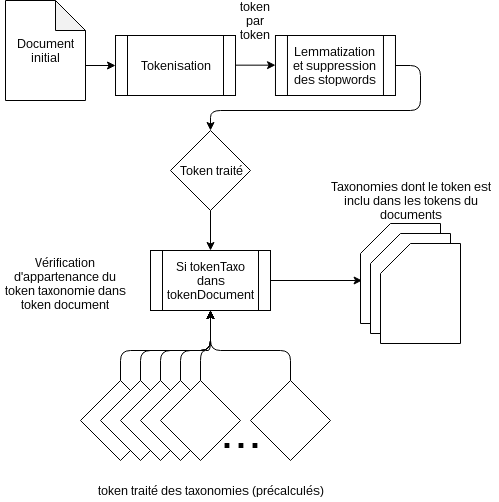
\includegraphics[width=0.7\textwidth]{diagFinalTaxo.png}
	\caption[]{Schéma fonctionnel du module d'assignement taxonomique final}
	\label{taxoFinal}
\end{figure}

\subsubsection{Parcours de l'arbre taxonomique}
\begin{figure}[h!]
  \centering
  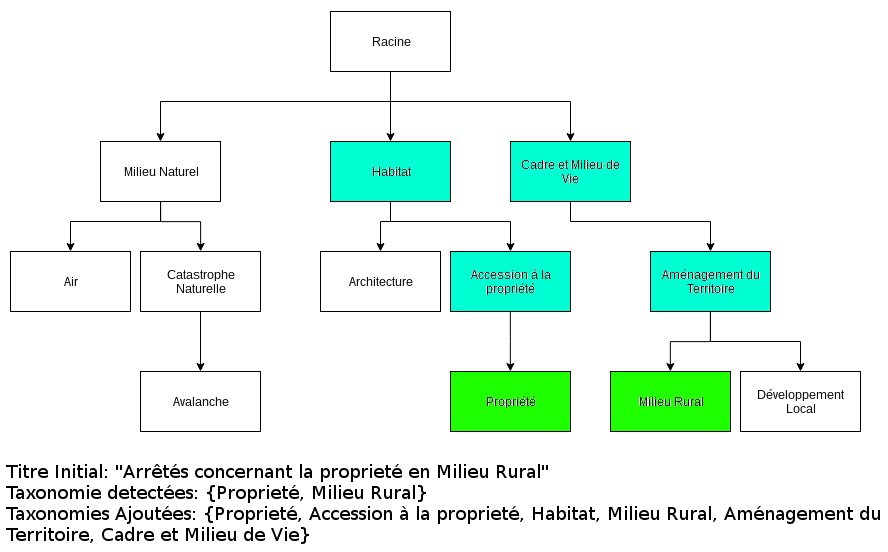
\includegraphics[width=\textwidth]{remontageArbre.png}
	\caption[]{Représentation de la technique de parcours d'arbre utilisée pour obtenir plus de taxonomies}
	\label{fig:tree}
\end{figure}


Pour obtenir une taxonomie plus vaste et contextuelle, nous prenons également en compte la structure de l'arbre taxonomique.
En effet, celle ci se présente sous forme d'un arbre dont un exemple de la structure est présenté en figure~\ref{fig:tree}. 
Chaque section possède des sous sections, qui permettent un affinage et une grande précision dans la classification.

L'idée centrale est de considérer que si un document possède comme taxonomie une feuille ou un noeud de cette arbre, alors il doit nécessairement posséder comme taxonomie tout les parents de ce noeud. 
Nous remontons alors jusqu'à la racine de l'arbre depuis le noeud de la taxonomie ayant été détectée, en ajoutant à la taxonomie du document tous les noeuds que nous rencontrons en chemin.
Cette approche nous permet d'obtenir une plus grande variété de taxonomie sans avoir à utiliser une analyse plus lourde sur le texte. 


\subsubsection{Classement des taxonomies}
En sortie, nous récupérons un grand nombre de taxonomie, données à la fois par la détection initiale et par le parcours de l'arbre.
Pour obtenir les taxonomies les plus représentatives du document, nous procédons ensuite à un classement des termes selon le nombre de fois ou chacune apparait dans le tableau des taxonomies.
Les taxonomies qui apparaissent souvent dans le document sont donc considérées comme plus `importante' que des taxonomies qui apparaissent plus rarement.

Le parcours d'arbre apportant une très grande quantité de nouveaux mots pour chaque taxonomie, il est donc nécessaire d'équilibrer ce système.
Pour se faire, nous appliquons un simple système de poids au taxonomies détectées: une taxonomie initiale aura un poids 100 supérieur à une taxonomie récupéré par le parcours d'arbre.

Cela permettra de garder uniquement les taxonomies les plus pertinentes.




Le résultat final se présente sous la forme d'un module python pouvant être importé et utilisé directement.



\subsection{Moteur de recherche}
Nous avons commencé la réalisation du moteur de recherche quand un fichier JSON test contenant 5 documents analysés fut disponible.
ElasticSearch et Kibana ont servit aux premiers tests fonctionnels, pour vérifier l'écriture de nos données et prendre en main l'utilisation d'ElasticSearch.

Nous avons ensuite réalisé une interface graphiquement avec l'aide AppBase.io, qui génère un code JavaScript basique, donnant la résultat de l'image~\ref{fig:firstSearch}:
\begin{figure}[h!]
  \centering
  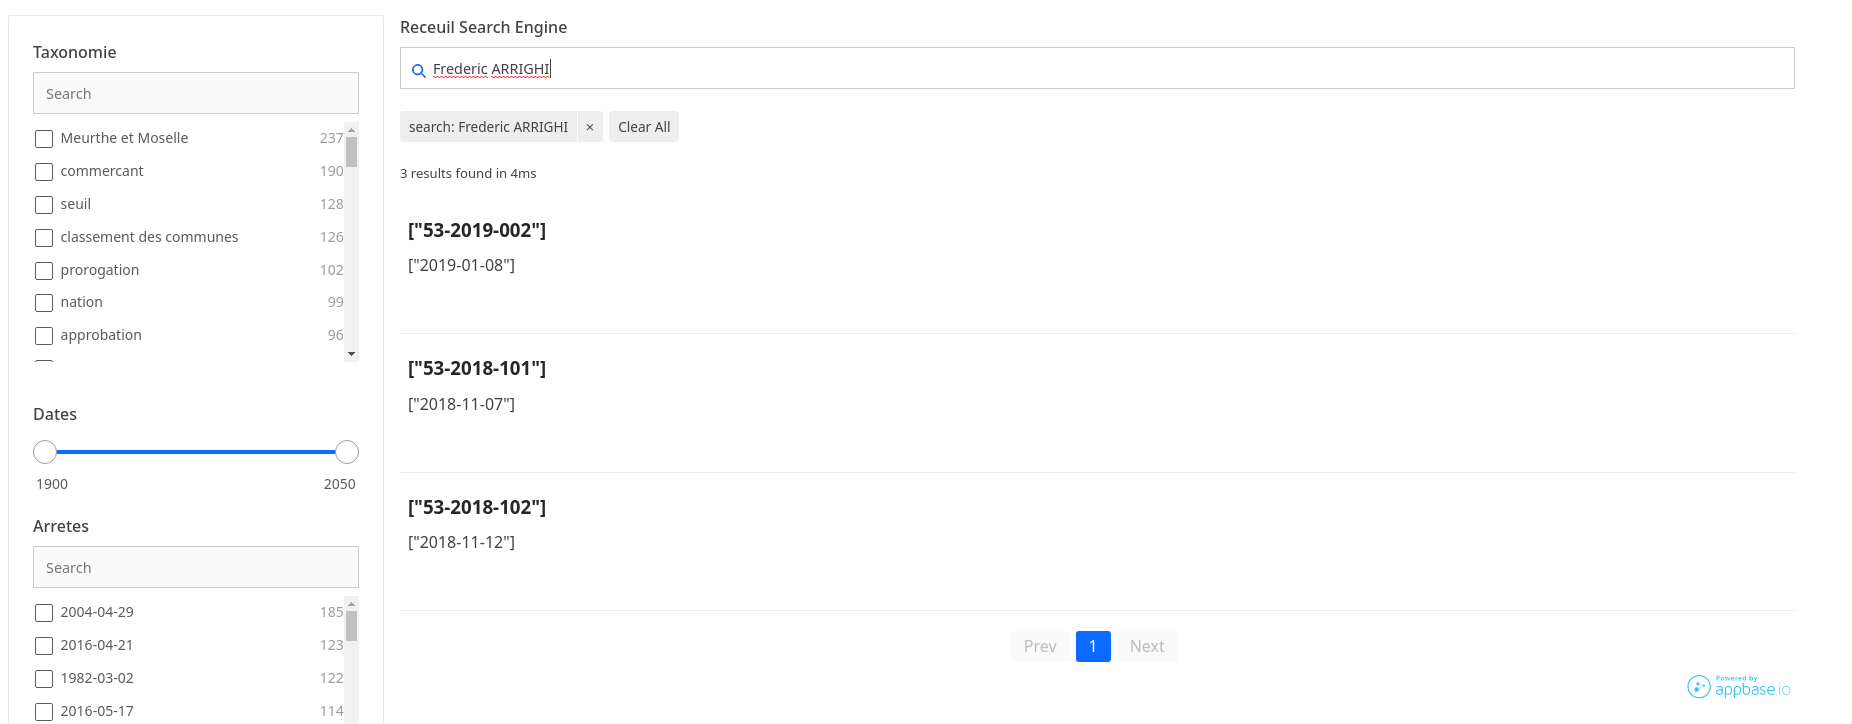
\includegraphics[width=\textwidth]{firstSearch.png}
	\caption[]{Premier moteur de recherche}
	\label{fig:firstSearch}
\end{figure}

Le code à ensuite été récupéré pour être amélioré localement.
Nous nous somme alors basés sur un Use Case déterminé précédemment et sur les retours de notre commanditaire pour améliorer l'interface et les systèmes de filtre et de d'affichage des résultats, en mettant par exemple les 4 taxonomies les plus pertinentes et un lien vers le transcript du document.

Pour cette version, nous n'avons pas pu mettre le lien vers le document directement cité sur le site de la prefecture car le format des url du site de la prefecture ne nous permettais pas un accès simple vers les documents.
La version actuelle du moteur de recherche donne donc uniquement un lien vers le transcript du document que nous avons placé sur Github.


\begin{figure}[h!]
  \centering
  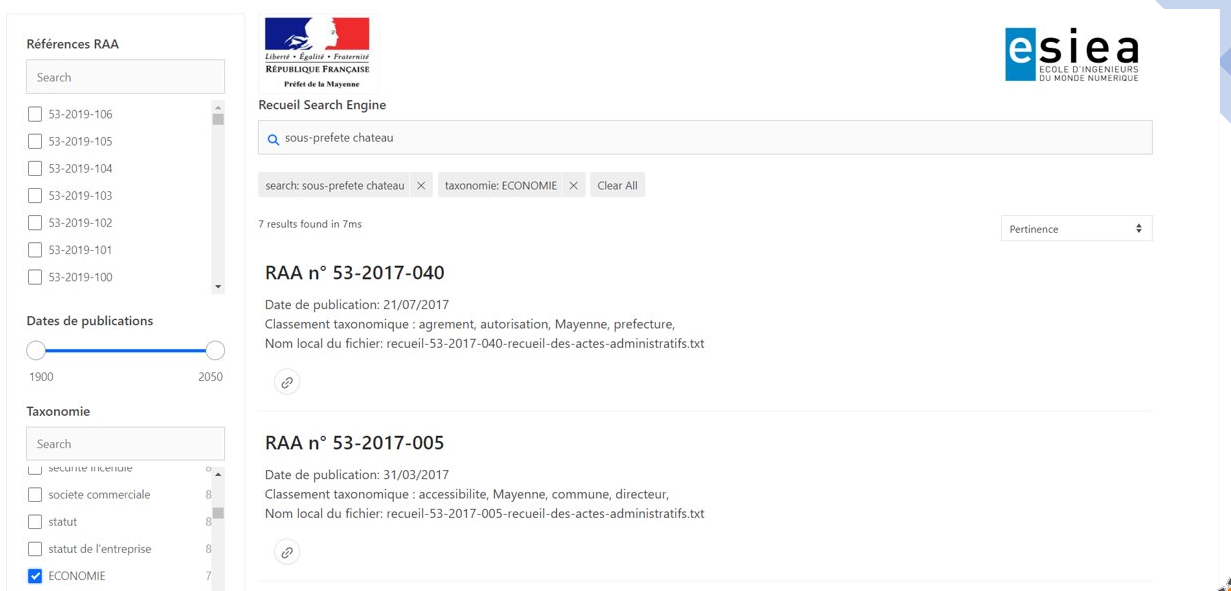
\includegraphics[width=\textwidth]{finalSearch.png}
	\caption[]{Moteur de recherche final}
	\label{fig:finalSearch}
\end{figure}

Cette version est bien meilleure pour un POC destiné à être montré à un public non initié, qui favorisera un support visuel agréable pour l'acceptation d'un projet.










